% Für Bindekorrektur als optionales Argument "BCORfaktormitmaßeinheit", dann
% sieht auch Option "twoside" vernünftig aus
% Näheres zu "scrartcl" bzw. "scrreprt" und "scrbook" siehe KOMA-Skript Doku
\documentclass[12pt,a4paper,titlepage,headinclude,bibtotoc]{scrartcl}


%---- Allgemeine Layout Einstellungen ------------------------------------------

% Für Kopf und Fußzeilen, siehe auch KOMA-Skript Doku
\usepackage[komastyle]{scrpage2}
\pagestyle{scrheadings}
\automark[section]{chapter}
\setheadsepline{0.5pt}[\color{black}]

%keine Einrückung
\parindent0pt

%Einstellungen für Figuren- und Tabellenbeschriftungen
\setkomafont{captionlabel}{\sffamily\bfseries}
\setcapindent{0em}


%---- Weitere Pakete -----------------------------------------------------------
% Die Pakete sind alle in der TeX Live Distribution enthalten. Wichtige Adressen
% www.ctan.org, www.dante.de

% Sprachunterstützung
\usepackage[ngerman]{babel}

% Benutzung von Umlauten direkt im Text
% entweder "latin1" oder "utf8"
\usepackage[utf8]{inputenc}

% Pakete mit Mathesymbolen und zur Beseitigung von Schwächen der Mathe-Umgebung
\usepackage{latexsym,exscale,amssymb,amsmath}

% Weitere Symbole
\usepackage[nointegrals]{wasysym}
\usepackage{eurosym}

% Anderes Literaturverzeichnisformat
%\usepackage[square,sort&compress]{natbib}

% Für Farbe
\usepackage{color}

% Zur Graphikausgabe
%Beipiel: \includegraphics[width=\textwidth]{grafik.png}
\usepackage{graphicx}

% Text umfließt Graphiken und Tabellen
% Beispiel:
% \begin{wrapfigure}[Zeilenanzahl]{"l" oder "r"}{breite}
%   \centering
%   \includegraphics[width=...]{grafik}
%   \caption{Beschriftung} 
%   \label{fig:grafik}
% \end{wrapfigure}
\usepackage{wrapfig}

% Mehrere Abbildungen nebeneinander
% Beispiel:
% \begin{figure}[htb]
%   \centering
%   \subfigure[Beschriftung 1\label{fig:label1}]
%   {\includegraphics[width=0.49\textwidth]{grafik1}}
%   \hfill
%   \subfigure[Beschriftung 2\label{fig:label2}]
%   {\includegraphics[width=0.49\textwidth]{grafik2}}
%   \caption{Beschriftung allgemein}
%   \label{fig:label-gesamt}
% \end{figure}
\usepackage{subfigure}

% Caption neben Abbildung
% Beispiel:
% \sidecaptionvpos{figure}{"c" oder "t" oder "b"}
% \begin{SCfigure}[rel. Breite (normalerweise = 1)][hbt]
%   \centering
%   \includegraphics[width=0.5\textwidth]{grafik.png}
%   \caption{Beschreibung}
%   \label{fig:}
% \end{SCfigure}
\usepackage{sidecap}

% Befehl für "Entspricht"-Zeichen
\newcommand{\corresponds}{\ensuremath{\mathrel{\widehat{=}}}}

%Für chemische Formeln (von www.dante.de)
%% Anpassung an LaTeX(2e) von Bernd Raichle
\makeatletter
\DeclareRobustCommand{\chemical}[1]{%
  {\(\m@th
   \edef\resetfontdimens{\noexpand\)%
       \fontdimen16\textfont2=\the\fontdimen16\textfont2
       \fontdimen17\textfont2=\the\fontdimen17\textfont2\relax}%
   \fontdimen16\textfont2=2.7pt \fontdimen17\textfont2=2.7pt
   \mathrm{#1}%
   \resetfontdimens}}
\makeatother

%Si Einheiten
\usepackage{siunitx}

%c++ Code einbinden
\usepackage{listings}
\lstset{numbers=left, numberstyle=\tiny, numbersep=5pt}

%Differential
\newcommand{\dif}{\ensuremath{\mathrm{d}}}

%Boxen,etc.
\usepackage{fancybox}
\usepackage{empheq}

%Fußnoten auf gleiche Seite
\interfootnotelinepenalty=1000

%Bibliography \bibliography{literatur} und \cite{gerthsen}
%\usepackage{cite}
\usepackage{babelbib}
\selectbiblanguage{ngerman}


\begin{document}

\begin{titlepage}
\centering
\textsc{\Large Anfängerpraktikum der Fakultät für
  Physik,\\[1.5ex] Universität Göttingen}

\vspace*{4.2cm}

\rule{\textwidth}{1pt}\\[0.5cm]
{\huge \bfseries
  Dampfdruck von Wasser\\[1.5ex]
  Protokoll:}\\[0.5cm]
\rule{\textwidth}{1pt}

\vspace*{3.0cm}

\begin{Large}
\begin{tabular}{ll}
Praktikant:
%	&  Skrollan Detzler\\
 	&  Felix Kurtz\\
 	&  Michael Lohmann\\
%	&  Kevin Lüdemann\\

  E-Mail: 
%	&  skrollan.detzler@stud.uni-goettingen.de\\
	&  felix.kurtz@stud.uni-goettingen.de\\
	& m.lohmann@stud.uni-goettingen.de\\	
%	&  kevin.luedemann@stud.uni-goettingen.de\\

 Betreuer: & Martin Ochmann\\
 Versuchsdatum: & 23.06.2014\\
\end{tabular}
\end{Large}

\vspace*{0.8cm}

\begin{Large}
\fbox{
  \begin{minipage}[t][2.5cm][t]{6cm} 
    Testat:
  \end{minipage}
}
\end{Large}

\end{titlepage}

\tableofcontents

\newpage

\section{Einleitung}
\label{sec:einleitung}

\section{Theorie}
\label{sec:theorie}

\subsection{Van-der-Waals-Gleichung}
Die reale Gasgleichung lautet nach \cite[S. 303]{gerthsen} mit der Ersetzung von $V_\text{mol}=V/n$ 
\begin{align}
	\left(p+\frac{n^2a}{V^2}\right)\left( V-nb \right)=nRT \label{eq:vanderwaalsgl}
\end{align}
Dabei betragen für Wasser die \emph{Van-der-Waals-Konstanten} $a=0.5537\si{\pascal~\meter^6}$ (Binnendruck) und $b=3.05\cdot10^{-5}\si{\meter^3}$ (Sättigungsdruck).\\
Sie entsteht dadurch, dass bei realen Gasen die Ausdehnung der Atome nicht mehr vernachlässigt wird.
Dadurch ist das "reale Volumen" größer, als das ideale und zwar um eine stoffabhängige Konstante multipliziert mit der Stoffmenge: $V_\text{ideal}=V_\text{Real}-n\cdot b$ .\\
Da in der idealen Gasgleichung die intermolekularen Kräfte bis auf elastische Stöße vernachlässigt sind, muss auch im Druck ein Korrekturfaktor eingeführt werden.
Der Druck sinkt durch die zusätzlichen Möglichkeiten, Energie an andere Teilchen zu übertragen, weshalb zu dem "realen Druck" ein Summand hinzugefügt werden muss, um den idealen zu bekommen: $p_\text{ideal}=p_\text{real}+\frac{n^2\cdot a^2}{V^2}$ .
Aus der idealen Gasgleichung $p_\text{ideal}V_\text{ideal}=nRT$ wird so Gleichung \eqref{eq:vanderwaalsgl}.


\subsection{Maxwell'sche Gerade}
Diskutiert man die Kurven, die sich aus der Van-der-Waals-Gleichung ergeben, so stellt man leicht fest, dass die Kurven für hohe Temperaturen einer Hyperbel entsprechen.
Für kleinere Temperaturen weicht die Kurve aber immer mehr von der Hyperbel ab und unterhalb einer kritischen Temperatur $T_k$ besitzt sie sogar zwei Extrempunkte.
Da ein Gas somit bei einer Temperatur einen bestimmten Druck bei mehreren Volumina annehmen kann, könnte man damit ein \emph{Perpetuum Mobile} 2. Art bauen.
Der 2. Hauptsatz der Thermodynamik verbietet dies jedoch und so führte Maxwell eine Korrekturgerade für diesen Bereich ein.
Er forderte, dass eine waagerechte Gerade so in diesen Bereich eingepasst wurde, dass der Flächeninhalt zwischen Gerade und Van-der-Waals-Gleichung in beiden Abschnitten gleich groß ist.
Diese Gerade erhilt ihm zu ehren den Namen \emph{Maxwell Gerade}.


\subsection{Carnot'scher Kreisprozess}

\subsection{Clausius-Clapeyron-Gleichung}

\subsection{Widerstandsthermometer}

\section{Durchführung}
\label{sec:durchfuehrung}
\begin{figure}[!htb]
	\centering
	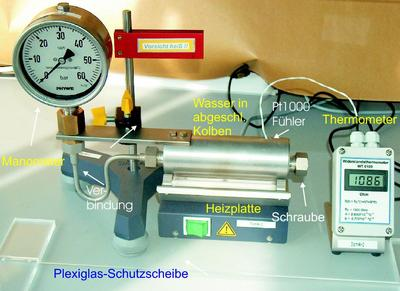
\includegraphics[scale=1.0]{Aufbau.jpg}
	\caption{Versuchsaufbau Quelle:LP}	
	\label{fig:Aufbau}
\end{figure}

Nachdem die Sicherheitshinweise (insbesondere die starke Erwärmung steigert das Gefahrenpotential) sorgfältig durchgelesen wurden, schaltet man das Gerät ein.
Der Heizstrahler erwärmt dann den mit Wasser gefüllten Kolben, welches dadurch verdampft.
Am angeschlossenen Manometer liest man den Druck ab.
Zeitgleich notiert man den Wert des Widerstandsthermometers und somit indirekt die Temperatur.
Dies geschieht in 1 Bar-Schritten.
Das Heizen wird beendet, wenn $1900 ~\si{\ohm}$ oder $45 \si{\bar}$ überschritten werden, damit das Gerät keinen Schaden nimmt.
Nun wird die Messung während des Abkühlens wiederholt.

\subsection{Sicherheitshinweise}


\section{Auswertung}
\label{sec:auswertung}
\subsection{Druckkurven}
\begin{table}
 \centering
 \begin{tabular}{|c|c|}
   \hline
   R$_0$ & $1000 ~ \si{\ohm}$\\
   A   & $3.9083 \cdot 10^{-3} ~ \si{\celsius^{-1}}$\\
   B   & $-5.775 \cdot 10^{-7} ~ \si{\celsius^{-2}}$\\
   \hline
 \end{tabular}
 \caption{Kennwerte des Widerstandsthermometers}
 \label{tab:Pt1000}
\end{table}

\begin{align}
	R(\vartheta)&=R_0\cdot\left(1 + A\vartheta + B\vartheta^2\right)\\ \Rightarrow
	\vartheta&=-\frac{A}{2B}-\sqrt{\frac{A^2}{4B^2}-\frac{1}{B}+\frac{R}{R_0 B}}
\end{align}
\begin{align}
	\Delta\vartheta=\pm (0.3~\si{\celsius}+0.005\vartheta)
\end{align}

Nun muss $\vartheta$ noch in Kelvin umgerechnet werden.
Außerdem wird für $p_0$ der gemessene Umgebungsdruck von 1017 hPa verwendet.

\begin{figure}[!htb]
	\centering
	% GNUPLOT: LaTeX picture with Postscript
\begingroup
  \makeatletter
  \providecommand\color[2][]{%
    \GenericError{(gnuplot) \space\space\space\@spaces}{%
      Package color not loaded in conjunction with
      terminal option `colourtext'%
    }{See the gnuplot documentation for explanation.%
    }{Either use 'blacktext' in gnuplot or load the package
      color.sty in LaTeX.}%
    \renewcommand\color[2][]{}%
  }%
  \providecommand\includegraphics[2][]{%
    \GenericError{(gnuplot) \space\space\space\@spaces}{%
      Package graphicx or graphics not loaded%
    }{See the gnuplot documentation for explanation.%
    }{The gnuplot epslatex terminal needs graphicx.sty or graphics.sty.}%
    \renewcommand\includegraphics[2][]{}%
  }%
  \providecommand\rotatebox[2]{#2}%
  \@ifundefined{ifGPcolor}{%
    \newif\ifGPcolor
    \GPcolortrue
  }{}%
  \@ifundefined{ifGPblacktext}{%
    \newif\ifGPblacktext
    \GPblacktexttrue
  }{}%
  % define a \g@addto@macro without @ in the name:
  \let\gplgaddtomacro\g@addto@macro
  % define empty templates for all commands taking text:
  \gdef\gplbacktext{}%
  \gdef\gplfronttext{}%
  \makeatother
  \ifGPblacktext
    % no textcolor at all
    \def\colorrgb#1{}%
    \def\colorgray#1{}%
  \else
    % gray or color?
    \ifGPcolor
      \def\colorrgb#1{\color[rgb]{#1}}%
      \def\colorgray#1{\color[gray]{#1}}%
      \expandafter\def\csname LTw\endcsname{\color{white}}%
      \expandafter\def\csname LTb\endcsname{\color{black}}%
      \expandafter\def\csname LTa\endcsname{\color{black}}%
      \expandafter\def\csname LT0\endcsname{\color[rgb]{1,0,0}}%
      \expandafter\def\csname LT1\endcsname{\color[rgb]{0,1,0}}%
      \expandafter\def\csname LT2\endcsname{\color[rgb]{0,0,1}}%
      \expandafter\def\csname LT3\endcsname{\color[rgb]{1,0,1}}%
      \expandafter\def\csname LT4\endcsname{\color[rgb]{0,1,1}}%
      \expandafter\def\csname LT5\endcsname{\color[rgb]{1,1,0}}%
      \expandafter\def\csname LT6\endcsname{\color[rgb]{0,0,0}}%
      \expandafter\def\csname LT7\endcsname{\color[rgb]{1,0.3,0}}%
      \expandafter\def\csname LT8\endcsname{\color[rgb]{0.5,0.5,0.5}}%
    \else
      % gray
      \def\colorrgb#1{\color{black}}%
      \def\colorgray#1{\color[gray]{#1}}%
      \expandafter\def\csname LTw\endcsname{\color{white}}%
      \expandafter\def\csname LTb\endcsname{\color{black}}%
      \expandafter\def\csname LTa\endcsname{\color{black}}%
      \expandafter\def\csname LT0\endcsname{\color{black}}%
      \expandafter\def\csname LT1\endcsname{\color{black}}%
      \expandafter\def\csname LT2\endcsname{\color{black}}%
      \expandafter\def\csname LT3\endcsname{\color{black}}%
      \expandafter\def\csname LT4\endcsname{\color{black}}%
      \expandafter\def\csname LT5\endcsname{\color{black}}%
      \expandafter\def\csname LT6\endcsname{\color{black}}%
      \expandafter\def\csname LT7\endcsname{\color{black}}%
      \expandafter\def\csname LT8\endcsname{\color{black}}%
    \fi
  \fi
  \setlength{\unitlength}{0.0500bp}%
  \begin{picture}(7200.00,5040.00)%
    \gplgaddtomacro\gplbacktext{%
      \csname LTb\endcsname%
      \put(946,704){\makebox(0,0)[r]{\strut{}-0.5}}%
      \put(946,1156){\makebox(0,0)[r]{\strut{} 0}}%
      \put(946,1609){\makebox(0,0)[r]{\strut{} 0.5}}%
      \put(946,2061){\makebox(0,0)[r]{\strut{} 1}}%
      \put(946,2513){\makebox(0,0)[r]{\strut{} 1.5}}%
      \put(946,2966){\makebox(0,0)[r]{\strut{} 2}}%
      \put(946,3418){\makebox(0,0)[r]{\strut{} 2.5}}%
      \put(946,3870){\makebox(0,0)[r]{\strut{} 3}}%
      \put(946,4323){\makebox(0,0)[r]{\strut{} 3.5}}%
      \put(946,4775){\makebox(0,0)[r]{\strut{} 4}}%
      \put(1078,484){\makebox(0,0){\strut{} 1.9}}%
      \put(1714,484){\makebox(0,0){\strut{} 2}}%
      \put(2350,484){\makebox(0,0){\strut{} 2.1}}%
      \put(2986,484){\makebox(0,0){\strut{} 2.2}}%
      \put(3622,484){\makebox(0,0){\strut{} 2.3}}%
      \put(4259,484){\makebox(0,0){\strut{} 2.4}}%
      \put(4895,484){\makebox(0,0){\strut{} 2.5}}%
      \put(5531,484){\makebox(0,0){\strut{} 2.6}}%
      \put(6167,484){\makebox(0,0){\strut{} 2.7}}%
      \put(6803,484){\makebox(0,0){\strut{} 2.8}}%
      \put(176,2739){\rotatebox{-270}{\makebox(0,0){\strut{}$\ln(\frac{p}{p_0})$}}}%
      \put(3940,154){\makebox(0,0){\strut{}$1/T~[\si{10^{-3}/\kelvin}]$}}%
    }%
    \gplgaddtomacro\gplfronttext{%
      \csname LTb\endcsname%
      \put(5816,4602){\makebox(0,0)[r]{\strut{}Messwerte}}%
      \csname LTb\endcsname%
      \put(5816,4382){\makebox(0,0)[r]{\strut{}Regressionsgerade}}%
    }%
    \gplbacktext
    \put(0,0){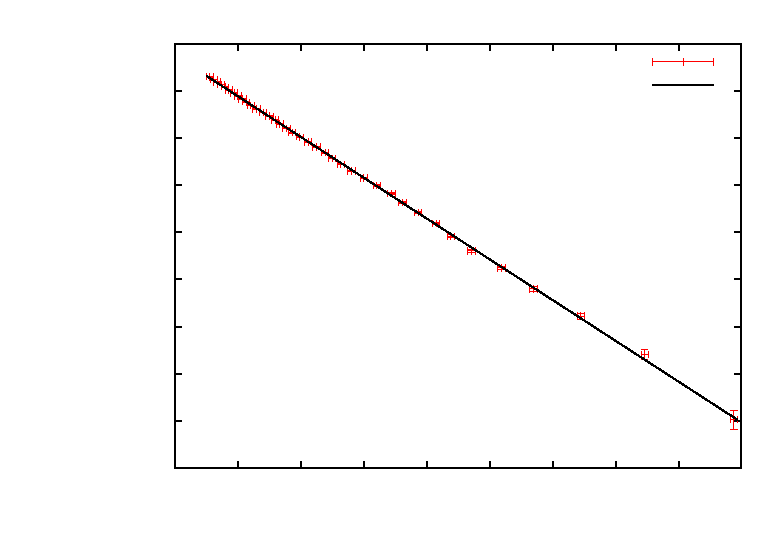
\includegraphics{Erwaermen}}%
    \gplfronttext
  \end{picture}%
\endgroup

	\caption{Arrheniusplot für das Erwärmen}
	\label{fig:mess1}
\end{figure}

\begin{figure}[!htb]
	\centering
	% GNUPLOT: LaTeX picture with Postscript
\begingroup
  \makeatletter
  \providecommand\color[2][]{%
    \GenericError{(gnuplot) \space\space\space\@spaces}{%
      Package color not loaded in conjunction with
      terminal option `colourtext'%
    }{See the gnuplot documentation for explanation.%
    }{Either use 'blacktext' in gnuplot or load the package
      color.sty in LaTeX.}%
    \renewcommand\color[2][]{}%
  }%
  \providecommand\includegraphics[2][]{%
    \GenericError{(gnuplot) \space\space\space\@spaces}{%
      Package graphicx or graphics not loaded%
    }{See the gnuplot documentation for explanation.%
    }{The gnuplot epslatex terminal needs graphicx.sty or graphics.sty.}%
    \renewcommand\includegraphics[2][]{}%
  }%
  \providecommand\rotatebox[2]{#2}%
  \@ifundefined{ifGPcolor}{%
    \newif\ifGPcolor
    \GPcolortrue
  }{}%
  \@ifundefined{ifGPblacktext}{%
    \newif\ifGPblacktext
    \GPblacktexttrue
  }{}%
  % define a \g@addto@macro without @ in the name:
  \let\gplgaddtomacro\g@addto@macro
  % define empty templates for all commands taking text:
  \gdef\gplbacktext{}%
  \gdef\gplfronttext{}%
  \makeatother
  \ifGPblacktext
    % no textcolor at all
    \def\colorrgb#1{}%
    \def\colorgray#1{}%
  \else
    % gray or color?
    \ifGPcolor
      \def\colorrgb#1{\color[rgb]{#1}}%
      \def\colorgray#1{\color[gray]{#1}}%
      \expandafter\def\csname LTw\endcsname{\color{white}}%
      \expandafter\def\csname LTb\endcsname{\color{black}}%
      \expandafter\def\csname LTa\endcsname{\color{black}}%
      \expandafter\def\csname LT0\endcsname{\color[rgb]{1,0,0}}%
      \expandafter\def\csname LT1\endcsname{\color[rgb]{0,1,0}}%
      \expandafter\def\csname LT2\endcsname{\color[rgb]{0,0,1}}%
      \expandafter\def\csname LT3\endcsname{\color[rgb]{1,0,1}}%
      \expandafter\def\csname LT4\endcsname{\color[rgb]{0,1,1}}%
      \expandafter\def\csname LT5\endcsname{\color[rgb]{1,1,0}}%
      \expandafter\def\csname LT6\endcsname{\color[rgb]{0,0,0}}%
      \expandafter\def\csname LT7\endcsname{\color[rgb]{1,0.3,0}}%
      \expandafter\def\csname LT8\endcsname{\color[rgb]{0.5,0.5,0.5}}%
    \else
      % gray
      \def\colorrgb#1{\color{black}}%
      \def\colorgray#1{\color[gray]{#1}}%
      \expandafter\def\csname LTw\endcsname{\color{white}}%
      \expandafter\def\csname LTb\endcsname{\color{black}}%
      \expandafter\def\csname LTa\endcsname{\color{black}}%
      \expandafter\def\csname LT0\endcsname{\color{black}}%
      \expandafter\def\csname LT1\endcsname{\color{black}}%
      \expandafter\def\csname LT2\endcsname{\color{black}}%
      \expandafter\def\csname LT3\endcsname{\color{black}}%
      \expandafter\def\csname LT4\endcsname{\color{black}}%
      \expandafter\def\csname LT5\endcsname{\color{black}}%
      \expandafter\def\csname LT6\endcsname{\color{black}}%
      \expandafter\def\csname LT7\endcsname{\color{black}}%
      \expandafter\def\csname LT8\endcsname{\color{black}}%
    \fi
  \fi
  \setlength{\unitlength}{0.0500bp}%
  \begin{picture}(7200.00,5040.00)%
    \gplgaddtomacro\gplbacktext{%
      \csname LTb\endcsname%
      \put(1386,704){\makebox(0,0)[r]{\strut{} 12}}%
      \put(1386,1286){\makebox(0,0)[r]{\strut{} 12.5}}%
      \put(1386,1867){\makebox(0,0)[r]{\strut{} 13}}%
      \put(1386,2449){\makebox(0,0)[r]{\strut{} 13.5}}%
      \put(1386,3031){\makebox(0,0)[r]{\strut{} 14}}%
      \put(1386,3613){\makebox(0,0)[r]{\strut{} 14.5}}%
      \put(1386,4194){\makebox(0,0)[r]{\strut{} 15}}%
      \put(1386,4776){\makebox(0,0)[r]{\strut{} 15.5}}%
      \put(1518,484){\makebox(0,0){\strut{} 0.0019}}%
      \put(2295,484){\makebox(0,0){\strut{} 0.002}}%
      \put(3072,484){\makebox(0,0){\strut{} 0.0021}}%
      \put(3849,484){\makebox(0,0){\strut{} 0.0022}}%
      \put(4627,484){\makebox(0,0){\strut{} 0.0023}}%
      \put(5404,484){\makebox(0,0){\strut{} 0.0024}}%
      \put(6181,484){\makebox(0,0){\strut{} 0.0025}}%
      \put(6958,484){\makebox(0,0){\strut{} 0.0026}}%
      \put(484,2740){\rotatebox{90}{\makebox(0,0){\strut{}$\ln(\frac{p}{\si{\pascal}})$}}}%
      \put(4238,154){\makebox(0,0){\strut{}$1/T~[\si{1/\kelvin}]$}}%
    }%
    \gplgaddtomacro\gplfronttext{%
      \csname LTb\endcsname%
      \put(5971,4603){\makebox(0,0)[r]{\strut{}Messwerte}}%
      \csname LTb\endcsname%
      \put(5971,4383){\makebox(0,0)[r]{\strut{}Regressionsgerade}}%
    }%
    \gplbacktext
    \put(0,0){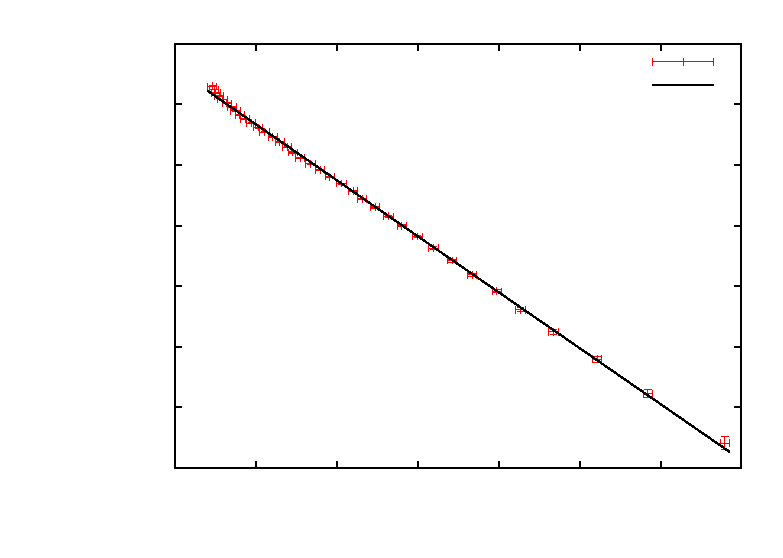
\includegraphics{Abkuehlen}}%
    \gplfronttext
  \end{picture}%
\endgroup

	\caption{Arrheniusplot für das Abkühlen}
	\label{fig:mess2}
\end{figure}

\begin{table}[!htb]
 \centering
 \begin{tabular}{|c|c|c|}
  \hline
  Größe&Erwärmen&Abkühlen\\
  \hline
  m & $(-4326 \pm 13)~\si{\kelvin}$ & $(-4618 \pm 21)~\si{\kelvin}$ \\
  b & $12.0672  \pm 0.02819$ & $12.5427 \pm 0.04496$ \\
  \hline
  %$\Lambda_V$ & $(35970 \pm 110)~\si{\joule/\mol}$ & $(38400 \pm 180)~\si{\joule/\mol}$\\
  %\hline
 \end{tabular}
 \label{tab:regErg}
\end{table}

Gewichtete Mittelwerte
\begin{align*}
 m=(-4407 \pm 11)~\si{\kelvin} \qquad
 b=12.201 \pm 0.024
\end{align*}

\begin{align*}
 \Lambda_V &= -m\cdot R\\
 \sigma_{\Lambda_V} &= \sigma_m \cdot R\\
 \Lambda_V&=(36640 \pm 100)~\si{\joule/\mol}
\end{align*}

\begin{align*}
 T_0 &= -\frac{m}{b}\\
 \sigma_{T_0} &= \sqrt{\left(\frac{\sigma_m}{b}\right)^2+\left(\frac{m\cdot \sigma_b}{b^2}\right)^2}\\
 T_0 &= (361.2 \pm 1.3)\si{\kelvin} = (88.0 \pm 1.3)\si{\celsius}
\end{align*}
Dampfdruck vun Wasser bei $T=0\si{\celsius}=273.15\si{\kelvin}$
\begin{align*}
 p &= p_0~\exp\left(m\frac{1}{T}+b\right)\\
 \sigma_p &= p~\sqrt{\frac{\sigma_m^2}{T^2}+\sigma_b^2}\\
 p &= (1990 \pm 100)\si{\pascal}
\end{align*}


\subsection{Siedetemperatur auf der Zugspitze}
barometrische Höhenformel
\begin{align}
 p(h)=p_0~\exp{\left(\frac{-\rho g h}{p_0}\right)}
\end{align}
\begin{align*}
 \frac{\Lambda_V}{R}\left(\frac{1}{T_0}-\frac{1}{T}\right)
\end{align*}

\begin{table}[!htb]
 \centering
 \begin{tabular}{|c|c|}
  \hline
  Größe & Wert\\
  \hline
  T$_0$ & $373.15~\si{\kelvin}$\\
  $\rho$ & $1.29~\si{\kilo \gram/\meter^3}$\\
  g & $9.81~\si{\meter/\second^2}$\\
  R & $8.31~\si{\joule/(\mol.\kelvin)}$\\
  $p_0$ & $1013.25~\si{\hecto \pascal}$\\
  $\Lambda_V$ & $40642 ~\si{\joule/\mol}$\\
  \hline
 \end{tabular}
 \caption{Literaturwerte}
 \label{tab:litW}
\end{table}
Höhe der Zugspitze $h=2962~\si{\meter}$
\begin{align*}
 T &= \left(\frac{1}{T_0}+\frac{\rho g h~R}{p_0~\Lambda_V}\right)^{-1}\\
 T&=362.9~\si{\kelvin}=89.8\si{\celsius}
\end{align*}




\section{Diskussion}
\label{sec:diskussion}

\section{Anhang}

\bibliography{literatur}
\bibliographystyle{babalpha}

\end{document}
